\documentclass[
	12pt,				% tamanho da fonte
    oneside,			% Oposto a twoside
	a4paper,			% tamanho do papel.
	english,			% idioma adicional para hifenização
	french,				% idioma adicional para hifenização
	spanish,			% idioma adicional para hifenização
	brazil				% o último idioma é o principal do documento
	]{abntex2}

\usepackage{lmodern}			% Usa a fonte Latin Modern			
\usepackage[T1]{fontenc}		% Selecao de codigos de fonte.
\usepackage[utf8]{inputenc}		% Codificacao do documento (conversão automática dos acentos)
\usepackage{lastpage}			% Usado pela Ficha catalográfica
\usepackage{indentfirst}		% Indenta o primeiro parágrafo de cada seção.
\usepackage{color}				% Controle das cores
\usepackage{graphicx}			% Inclusão de gráficos
\usepackage{microtype} 			% para melhorias de justificação
\usepackage{float} 			    % para fixação de imagens
\usepackage{caption}
\usepackage{lipsum}				% para geração de dummy text

\usepackage[brazilian,hyperpageref]{backref}	 % Paginas com as citações na bibl
\usepackage[alf]{abntex2cite}	% Citações padrão ABNT

\newcommand{\dd}[1]{\mathrm{d}#1}

% Pacote para a definição de novas cores
\usepackage{xcolor}
% Definindo novas cores
\definecolor{verde}{rgb}{0.25,0.5,0.35}
\definecolor{jpurple}{rgb}{0.5,0,0.35}
\definecolor{darkgreen}{rgb}{0.0, 0.2, 0.13}
% Configurando layout para mostrar codigos Java
\usepackage{listings}

\newcommand{\estiloC}{
\lstset{
    language=C,
    basicstyle=\ttfamily\small,
    keywordstyle=\color{jpurple}\bfseries,
    stringstyle=\color{red},
    commentstyle=\color{verde},
    morecomment=[s][\color{blue}]{/**}{*/},
    extendedchars=true,
    showspaces=false,
    showstringspaces=false,
    numbers=left,
    numberstyle=\tiny,
    breaklines=true,
    backgroundcolor=\color{cyan!10},
    breakautoindent=true,
    captionpos=b,
    xleftmargin=0pt,
    tabsize=2
}}

% ---
% Informações de dados para CAPA e FOLHA DE ROSTO
% ---
\titulo{Relatório de Estágio}
\autor{Felipe Marinho Tavares}
\data{Dezembro de 2018}
\local{Campinas -- São Paulo -- Brasil}
\instituicao{%
  Empresa: SAMSUNG ELETRÔNICA DA AMAZÔNIA
  \par
  Setor: Artificial Intelligence Research \& Development
  \par\par
  Supervisor: Ciro Cavani
  \par\par
  Engenharia de Computação
  \par
  Universidade Federal de Itajubá -- UNIFEI
  }
\tipotrabalho{Relatório de Estágio}
% O preambulo deve conter o tipo do trabalho, o objetivo,
% o nome da instituição e a área de concentração
% ---

% ---
% Configurações de aparência do PDF final

% alterando o aspecto da cor azul
\definecolor{blue}{RGB}{41,5,195}

% informações do PDF
\makeatletter
\hypersetup{
     	%pagebackref=true,
		pdftitle={\@title},
		pdfauthor={\@author},
    	pdfsubject={\imprimirpreambulo},
	    pdfcreator={LaTeX with abnTeX2},
		pdfkeywords={abnt}{latex}{abntex}{abntex2}{trabalho acadêmico},
		colorlinks=true,       		% false: boxed links; true: colored links
    	linkcolor=blue,          	% color of internal links
    	citecolor=blue,        		% color of links to bibliography
    	filecolor=magenta,      		% color of file links
		urlcolor=blue,
		bookmarksdepth=4
}
\makeatother
% ---

% ---
% Espaçamentos entre linhas e parágrafos
% ---

% O tamanho do parágrafo é dado por:
\setlength{\parindent}{1.3cm}

% Controle do espaçamento entre um parágrafo e outro:
\setlength{\parskip}{0.2cm}  % tente também \onelineskip

% ---
% compila o indice
% ---
\makeindex
% ---

% ----
% Início do documento
% ----
\begin{document}

% Seleciona o idioma do documento (conforme pacotes do babel)
%\selectlanguage{english}
\selectlanguage{brazil}

% Retira espaço extra obsoleto entre as frases.
\frenchspacing

% ----------------------------------------------------------
% ELEMENTOS PRÉ-TEXTUAIS
% ----------------------------------------------------------
% Capa e Folha de Rosto
\imprimircapa
\imprimirfolhaderosto*
% ---

% ---
% inserir o sumario
% ---
\pdfbookmark[0]{\contentsname}{toc}
\tableofcontents*
\clearpage
% ---

% ----------------------------------------------------------
% ELEMENTOS TEXTUAIS
% ----------------------------------------------------------
\textual

% ----------------------------------------------------------------
% Introdução e Conceitos Básicos *******************
% ----------------------------------------------------------------
\chapter{Introdução}

Este relatório busca descrever o período de estágio de 16/04/2018 à 31/12/2018 na empresa Samsung Eletrônica da Amazônia. O estágio supervisionado é componente curricular obrigatório junto à Universidade Federal de Itajubá. No curso de Engenharia de Computação, a carga horária necessária é de 196 horas.

A Samsung é um conglomerado multinacional de empresas. Destacando dentre elas a Samsung Electronics, referência na indústria de tecnologia de informação, eletrônicos de consumo e de semicondutores. Sua presença no Brasil é feita pela Samsung Eletrônica da Amazônia, que produz eletrônicos de consumo, e é uma empresa que faz uso da Lei da Informática (Lei nº 8.248, de 23 de outubro de 1991), qual fornece incentivos fiscais à empresas que conduzem práticas de pesquisa e desenvolvimento tecnológico no Brasil.

O aluno faz parte do centro Samsung Research Brazil (SRBR), foto na \autoref{fig:SRBR}, em Campinas - SP, no time de Artificial Intelligence Research \& Development (AI R\&D).

\begin{figure}[H]
  \centering
  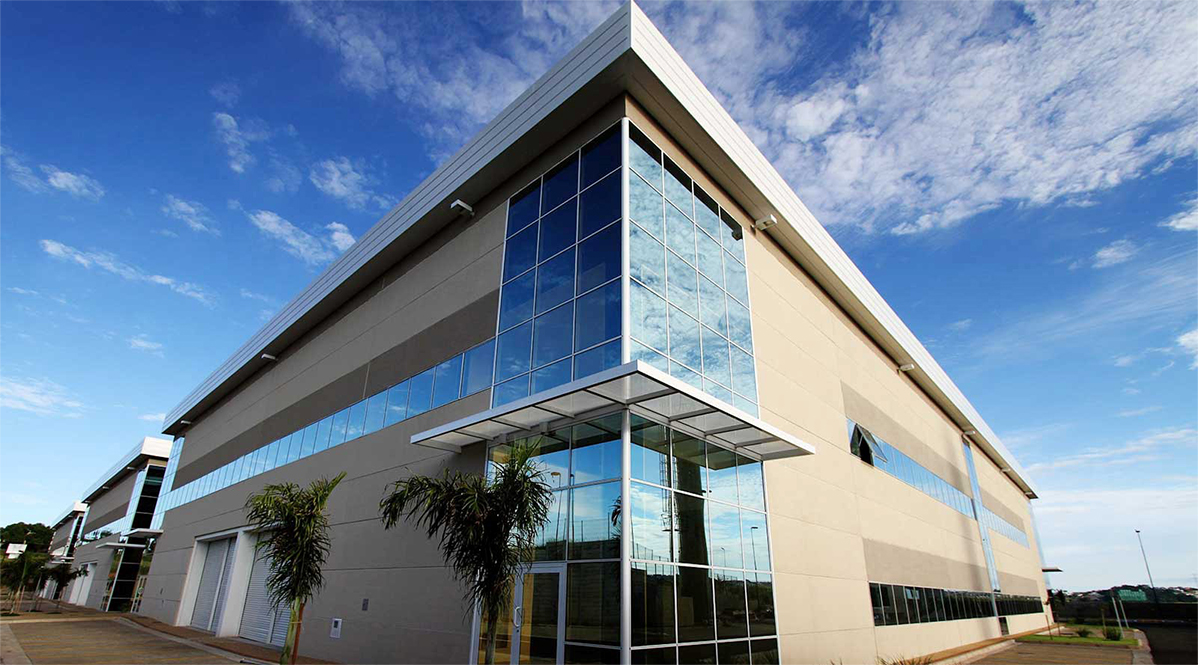
\includegraphics[width=400pt]{images/srbr-image.jpg}\\
  \caption[SRBR, Samsung Research Brazil]{SRBR, Samsung Research Brazil}
  \label{fig:SRBR}
\end{figure}

Desde a integração do estágio existe em efeito um \textit{Non-disclosure agreement} (NDA) no qual acordou-se a confidencialidade de informações proprietárias à empresa. Assim, o conteúdo desde relatório obrigatoriamente acata a não divulgação de informações confidenciais, e suficientemente descreve as atividades realizadas na empresa.

A SRBR desenvolve projetos de pesquisa e inovação com foco na melhoria e criação de produtos, obtenção de patentes, e contribuição à sociedade científica. Assim, com a realização de atividades que buscam por fim a concepção e melhoria de produtos e, por consequência, espelham padrões e práticas da indústria, é possível afirmar que o estágio cumpriu os objetivos firmados ao fornecer experiência e direcionamento profissional ao aluno.

\section{Contexto e Objetivos}

Samsung Research é o centro de pesquisa avançada das divisões de Consumer Electronics (CE) e IT \& Mobile Communications (IM), com uma rede global de 22 centros de pesquisa e desenvolvimento em 15 países, mostrado na \autoref{fig:samsung-research-network}. A SRBR, com aproximadamente 300 funcionários, está inserida nesta rede global sendo o único centro na América Latina, e busca continuamente se alinhar com a estratégia, visão, e tecnologias principais estabelecidas pela Samsung Research.

\begin{figure}[H] 
  \centering
  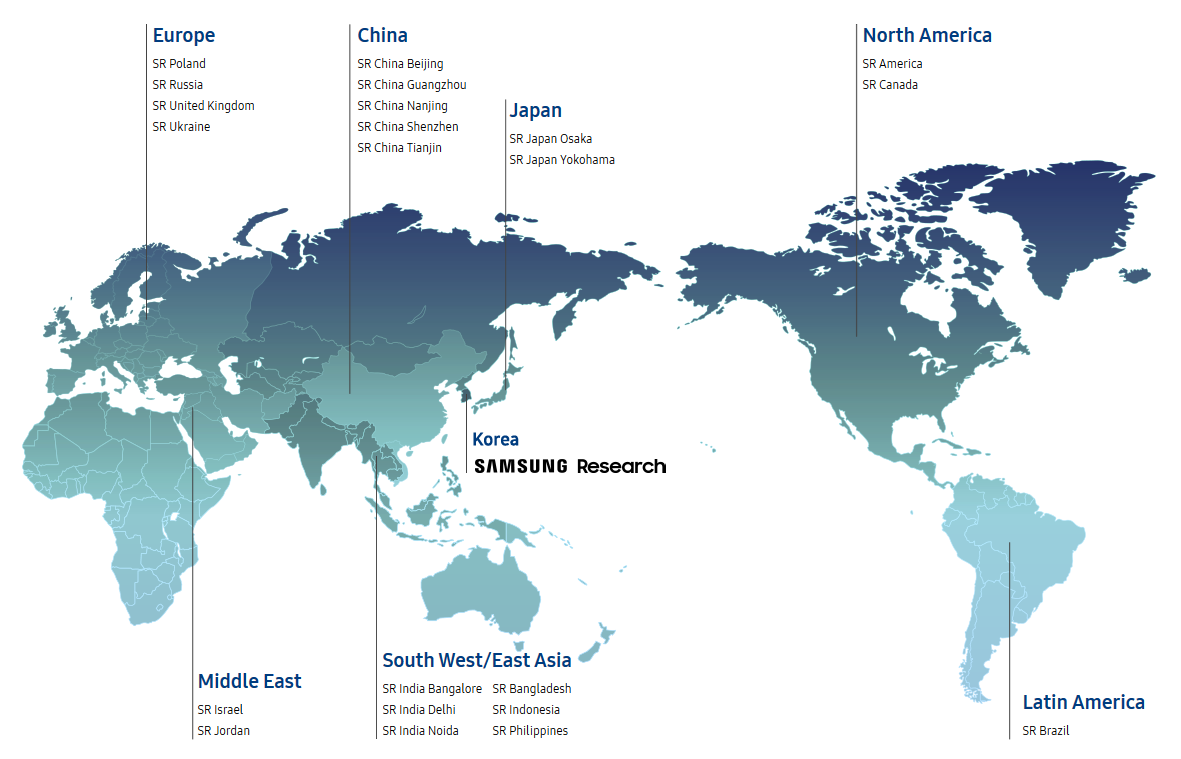
\includegraphics[width=400pt]{images/samsungresearch_centers.png}\\
  \caption[Samsung Global R&D Centers]{Samsung Global R\&D Centers}  \label{fig:samsung-research-network}
\end{figure}

Uma vez que a Lei da Informática é contribuinte direta da SRBR, um dos principais objetivos do centro brasileiro é de cultivar e manter o mercado local e continuamente contribuir para o desenvolvimento tecnológico e de pesquisa da região.

Na próxima seção as atividades de estágio realizadas na concedente serão exploradas.

% ----------------------------------------------------------------
% Metodologia *******************
% ----------------------------------------------------------------
\chapter{Atividades}

As atividades executadas ocorreram ao longo do ano de 2018, envolvendo, principalmente, funções de suporte a outros funcionários. Cada uma das atividades foi crucial no processo de aprendizado durante o estágio, melhorando conhecimentos profissionais e interpessoais, além de gerar uma melhor visão do funcionamento de uma empresa enquanto tendo impacto direto no desenvolvimento dos projetos em andamento.

De acordo com o termo de compromisso firmado com a concedente, as atividades planejadas de estágio são descritas em:
\begin{itemize}
    \item Prestar suporte na programação das atividades de pesquisa e desenvolvimento na área de inteligência artificial;
    \item Verificar os monitoramentos dos projetos;
    \item Verificar códigos de performance;
    \item Auxiliar na configuração de hardwares e softwares para experimentos.
\end{itemize}

Todas as atividades contaram com o acompanhamento de ao menos um tutor, que prestou suporte e solucionou eventuais dúvidas. Ainda foi necessário, entretanto, se familiarizar com o ambiente, descobrir e resolver problemas da maneira mais autodidata possível, com o intuito de não utilizar recursos sem a devida necessidade e, ao mesmo tempo, criar uma cultura de estudo pertinente à da empresa. 

Dessa maneira, a troca com a empresa aconteceu de maneira satisfatória, rendendo bons resultados para ambas as partes.

A descrição das atividades é separada em duas seções, respectivas à partição do aluno em dois diferentes projetos.

\section{Projeto 1}

A primeira atribuição do estágio foi a participação em um projeto que possui como um de seus objetivos analisar técnicas aplicadas em algoritmos de machine learning para determinados tipos de dispositivos, buscando melhorar uma métrica de desempenho (representação de execução mostrado na \autoref{fig:projeto1_diagram}).

\begin{figure}[H] 
  \centering
  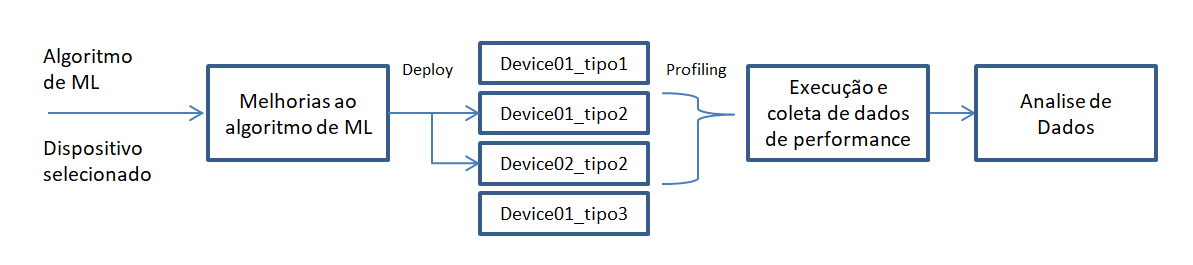
\includegraphics[width=450pt]{images/projeto1_diagram.png}\\
  \caption[Representação de execução, Projeto 1]{Representação de execução, Projeto 1}  \label{fig:projeto1_diagram}
\end{figure}

Atividades quanto ao desenvolvimento de artefatos de pesquisa nas etapa de deploy (configuração de dispositivos e execução) e profiling (coleta de dados) foram desenvolvidas pelo aluno a fim de validar as estratégias de implementação e documentar as abordagens para uso de outros membros do projeto. Os resultados das atividades foram registrados por meio de relatórios técnicos da pesquisa interna.

\section{Projeto 2}

Em um segundo momento o aluno foi atribuído à outro projeto com um dos objetivos de, a partir de uma base de dados, desenvolver um modelo de aprendizado de máquina para classificações de estados capaz de ser executado em uma implementação de um determinado dispositivo (representação do fluxo de desenvolvimento mostrado na \autoref{fig:projeto2_diagram}).  

\begin{figure}[H] 
  \centering
  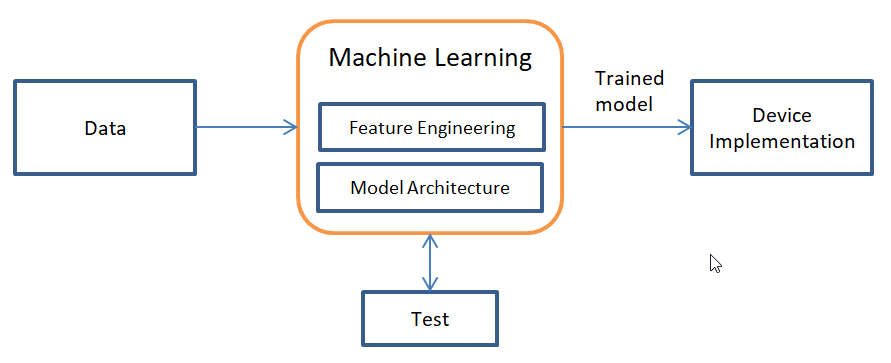
\includegraphics[width=400pt]{images/projeto2_diagram.png}\\
  \caption[Representação do fluxo de desenvolvimento, Projeto 2]{Representação do fluxo de desenvolvimento, Projeto 2}  \label{fig:projeto2_diagram}
\end{figure}

Houveram contribuições do aluno nas etapas de caracterização e extração de características dos dados (Feature Engineering), na concepção de arquiteturas, implementações e testes de modelos, e na implementação em dispositivo. Os artefatos gerados foram documentos por relatórios e compartilhados com equipes de outros R\&Ds.

% ----------------------------------------------------------
% CONCLUSÃO
% ----------------------------------------------------------
\chapter{Conclusão}

A experiência de estágio envolveu constante pesquisa e estudo para resolução de diversos problemas. Muitas vezes, foi necessária a comunicação com colegas para melhor entendimento do problema a ser resolvido. A responsabilidade tomada, por mais que limitada devido à posição, mostrou suficiente para que as atividades realizadas tivessem impacto no desenvolvimento de projetos. Dessa maneira, a imersão no ambiente empresarial se deu de maneira completa, com prazos a serem cumpridos e máximo desempenho objetivado.

O estágio apresentou caráter prático, representativo e adequado para a formação profissional devido à semelhança das atividades realizadas e o fluxo de trabalho da empresa. Além disso, para o desenvolvimento das atividades, o entendimento do contexto de trabalho, e manuseio de ferramentas fez-se uso de conhecimentos adquiridos durante a graduação e que foram aprimorados considerando agora outros problemas e soluções existentes na indústria.   

Por fim, durante toda a extensão dessas atividades, foi necessário o emprego de várias habilidades comportamentais, denominadas \textit{soft skills}. Essas habilidades envolvem capacidades interpessoais, e seu emprego é altamente desejado no ambiente de trabalho. Comportamentos de interesse geralmente envolvem proatividade, criatividade, gentileza, interesse e empenho ao se realizar atividades. Dessa maneira, todas as atividades empregadas durante o período de estágio tiveram, como embasamento, o emprego destes valores para que o ambiente de trabalho se mantivesse sempre saudável. A partir do retorno de colegas de trabalho, foi possível então aprender como se portar de maneira mais agradável e produtiva no ambiente empresarial, assim como descobrir pontos a serem trabalhados e aperfeiçoados.

% ----------------------------------------------------------
% ELEMENTOS PÓS-TEXTUAIS
% ----------------------------------------------------------
\postextual
% ----------------------------------------------------------

% ----------------------------------------------------------
% Referências bibliográficas
% ----------------------------------------------------------
%\bibliography{references}

\end{document}
